\documentclass[a4paper,12pt,oneside]{book}
\usepackage{polski}
\usepackage[utf8]{inputenc}
\usepackage{graphicx}
\graphicspath{{./images}}
\usepackage[shortlabels]{enumitem}
\usepackage{amssymb}
\usepackage{amsmath}
\usepackage{indentfirst}
\usepackage{pdfpages}

\usepackage{tikz}
%\usepackage{etoolbox} % for \ifthen
\usepackage{listofitems} % for \readlist to create arrays
\usetikzlibrary{arrows.meta} % for arrow size
\usepackage[outline]{contour} % glow around text
\contourlength{1.4pt}
\usepackage[margin=1in]{geometry}
\usepackage{listings}


\tikzset{>=latex} % for LaTeX arrow head
\usepackage{xcolor}
\colorlet{myred}{red!80!black}
\colorlet{myblue}{blue!80!black}
\colorlet{mygreen}{green!60!black}
\colorlet{myorange}{orange!70!red!60!black}
\colorlet{mydarkred}{red!30!black}
\colorlet{mydarkblue}{blue!40!black}
\colorlet{mydarkgreen}{green!30!black}
\tikzstyle{node}=[thick,circle,draw=myblue,minimum size=22,inner sep=0.5,outer sep=0.6]
\tikzstyle{node in}=[node,green!20!black,draw=mygreen!30!black,fill=mygreen!25]
\tikzstyle{node hidden}=[node,blue!20!black,draw=myblue!30!black,fill=myblue!20]
\tikzstyle{node convol}=[node,orange!20!black,draw=myorange!30!black,fill=myorange!20]
\tikzstyle{node out}=[node,red!20!black,draw=myred!30!black,fill=myred!20]
\tikzstyle{connect}=[thick,mydarkblue] %,line cap=round
\tikzstyle{connect arrow}=[-{Latex[length=4,width=3.5]},thick,mydarkblue,shorten <=0.5,shorten >=1]
\tikzset{ % node styles, numbered for easy mapping with \nstyle
	node 1/.style={node in},
	node 2/.style={node hidden},
	node 3/.style={node out},
}
\def\nstyle{int(\lay<\Nnodlen?min(2,\lay):3)} % map layer number onto 1, 2, or 3

\def\shrug{\texttt{\raisebox{0.75em}{\char`\_}\char`\\\char`\_\kern-0.5ex(\kern-0.25ex\raisebox{0.25ex}{\rotatebox{45}{\raisebox{-.75ex}"\kern-1.5ex\rotatebox{-90})}}\kern-0.5ex)\kern-0.5ex\char`\_/\raisebox{0.75em}{\char`\_}}}

\renewcommand\thechapter{\Roman{chapter}}
\renewcommand\thesection{\arabic{section}}
\renewcommand\thesubsection{\thesection.\arabic{subsection}}

\begin{document}

	
\includepdf{Odpowiedz-cover-page.pdf}

	\tableofcontents
	\newpage
	
	\chapter{Pytania - dr. hab. Bogdan Księżopolski}
	
		\section{Sieci i programowanie sieciowe}
			\subsection{Protokoły TCP i UDP - porównanie i zastosowanie.}
			
				\subsubsection*{TCP}
				
				Protokół TCP lub Transmission Control Protocol jest protokołem zorientowanym na połączenie, znajdującym się w warstwie transportowej modelu TCP / IP. Nawiązuje połączenie między komputerem źródłowym a docelowym przed rozpoczęciem komunikacji.
				
				\begin{figure}[h!]
					\centering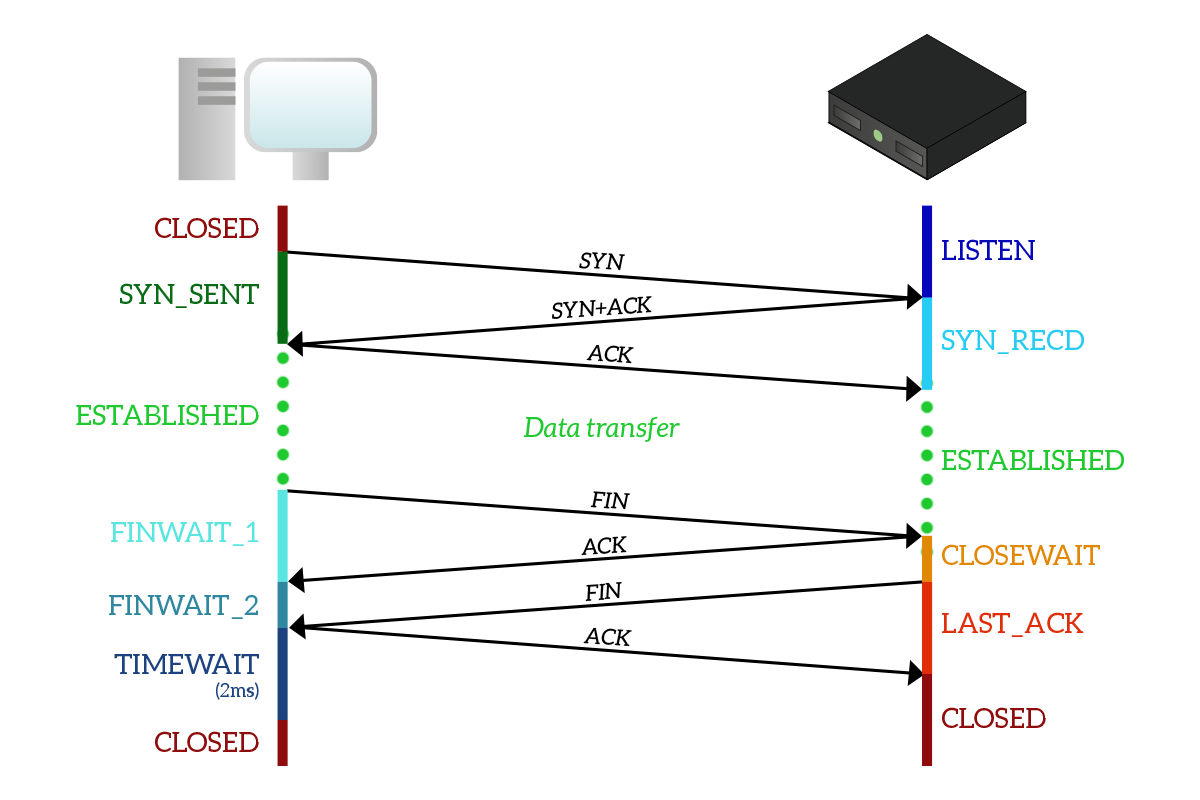
\includegraphics[scale=0.30]{tcp.png}
					\caption{TCP}
				\end{figure}
				
				Jest wysoce niezawodny, ponieważ wykorzystuje 3-drożną kontrolę uzgadniania, przepływu, błędu i przeciążenia. Zapewnia to, że dane wysyłane z komputera źródłowego są dokładnie odbierane przez komputer docelowy. Jeśli w przypadku, otrzymane dane nie są w odpowiednim formacie, to TCP ponownie przesyła dane.
				Poniższe protokoły używają TCP do transmisji danych:
				\begin{itemize}
					\item HTTP
					\item HTTPs
					\item FTP
					\item SMTP
				\end{itemize}
				
				\subsubsection*{UDP}
				
				\begin{figure}[h!]
					\centering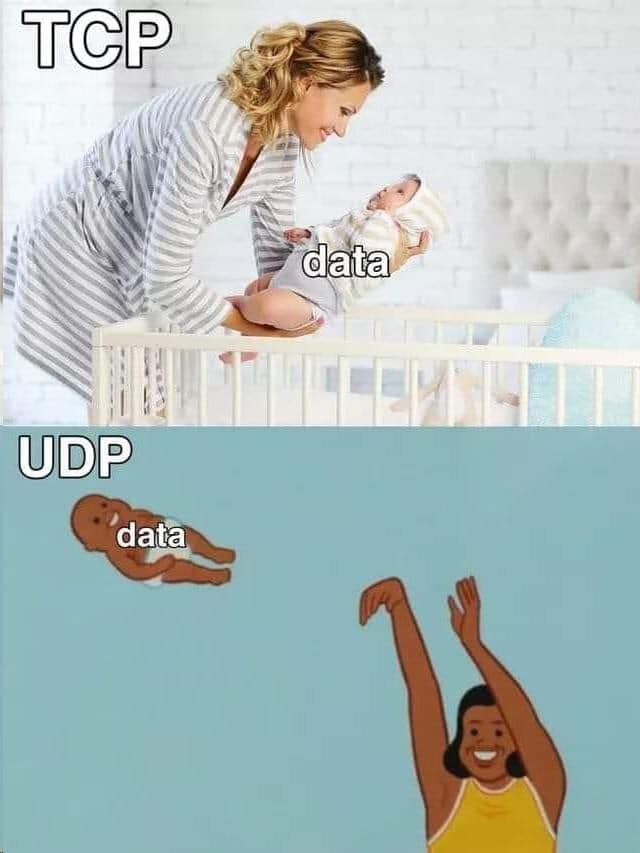
\includegraphics[scale=0.25]{udp.jpg}
					\caption{UDP :D}
				\end{figure}
				
				Protokół UDP lub User Datagram Protocol to bezpołączeniowy protokół znajdujący się w warstwie transportowej modelu TCP / IP. Nie ustanawia połączenia ani nie sprawdza, czy komputer docelowy jest gotowy do odbioru, czy też nie, po prostu przesyła dane bezpośrednio. Protokół UDP służy do przesyłania danych z większą szybkością. Jest mniej niezawodny i dlatego jest używany do przesyłania danych, takich jak pliki audio i wideo.
				UDP nie gwarantuje ani dostarczenia danych, ani nie przesyła utraconych pakietów.	
				
							
			
			\newpage\subsection{Protokół IP.}
				\subsubsection{IP (Internet Protocol)}
				Protokół internetowy jest protokołem komunikacyjnym warstwy Internet w modelu TCP/IP (odpowiada warstwie sieciowej modelu OSI). Protokół ten definiuje zasady i sposoby postępowania urządzeń sieciowych w celu nawiązania połączenia, utrzymania go i samej transmisji danych. Protokół IP stosowany jest w większości rodzajów sieci, w tym w sieci lokalnej i sieci Internet (każdy host, np. komputer, posiada swój własny, unikalny dla sieci adres IP).
				
				Dane z użyciem protokołu IP transmitowane są w pakietach (paczkach danych). Nie gwarantuje on jednak dotarcia danych do celu czy utrzymania kolejności pakietów. Może się zdążyć, ze odbiorca otrzyma kilkukrotnie ten sam pakiet z całej paczki danych, pakiety dotrą w innej kolejności lub nie dotrą w ogóle. W celu zapewnienia prawidłowej transmisji stosuje się różne techniki w wyższej warstwie, np. z użyciem protokołu TCP.
				
				Ponieważ każdy host w sieci posiada swój własny unikalny adres IP, obecnie wykorzystywana czwarta wersja protokołu (v4) okazała się niewystarczająca i brakuje wolnych adresów IP. W tym celu utworzona została wersja szósta (v6) znacznie zwiększająca ilość różnych adresów IP. Same adresy IP dzielone są na kilka grup z których 3 najważniejsze to adresy publiczne, adresy prywatne (do wykorzystania w sieciach domowych, np. 192.168.1.1), oraz adresy pętli zwrotnej (np. 127.0.0.1).
				
				W skrócie:
				\begin{itemize}
					\item protokół komunikacyjny z warstwy trzeciej (sieci)
					\item jest to protokół bezpołączeniowy
					\item głównym zadaniem tego protokołu jest przypisywanie każdemu urządzeniu
					sieciowemu adresu IP i wybór trasy w celu przesłania pakietów z danymi (w
					przypadku problemów w przesyłaniu pakietów protokół wybierze trasy alternatywne
					do przesłania pakietów)
					\item nie zapewnia dostarczania pakietów (nie posiada mechanizmów retransmisji, lecz na
					szczęście za to odpowiadają protokoły z warstw wyższych)
				\end{itemize}
			\subsubsection{Klasy IP}
				\begin{figure}[h!]
					\centering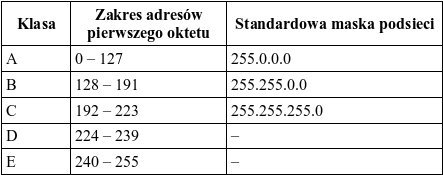
\includegraphics[scale=0.65]{ip-classes.jpg}
					\caption{Klasy IP}
				\end{figure}
			\subparagraph{Adresy klasy A} przeznaczone są dla dużych sieci. Pierwszy bit oktetu w którym zawarty jest adres sieci jest równy 0. W związku z tym adresy sieci mogą przyjmować wartości od 0 do 127. Sieci 0 i 127 są zarezerwowane, więc do wykorzystania pozostają sieci od 1 do 126. W każdej sieci należącej do klasy A możemy wyodrębnić 16777216 adresów (liczba urządzeń będzie o 2 mniejsza, ale o tym w dalszej części artykułu). Klasa 127.0.0.0 wykorzystywana jest na potrzeby pętli zwrotnej, tj. umożliwia wysyłanie pakietów do samego siebie. Maska standardowa dla tej klasy to 255.0.0.0.
			
			\subparagraph{Adresy klasy B} przeznaczone są do sieci średniej wielkości. Adres sieci zawarty jest w dwóch oktetach. Pierwsze dwa bity pierwszego oktetu wynoszą 10. W każdej sieci należącej do tego klasy można wyróżnić 65536 adresów (65534 urządzenia). Do tej klasy należą adresy sieci od 128 do 191 w ujęciu dziesiętnym. Maska standardowa dla tej klasy to 255.255.0.0.
			
			\subparagraph{Adresy klasy C} przeznaczone są dla małych sieci, gdyż każda sieć może posiadać „jedynie” 256 adresów (254 urządzenia). Na adres sieci w sieciach należących do tej klasy przeznaczone są 3 oktety. Pierwsze trzy bity adresu wynoszą 110, w związku z tym do klasy tej należą adresy od 192 do 223 dziesiętne. Maska standardowa dla tej klasy to 255.255.255.0.
			
			\subparagraph{Klasa D} została zarezerwowana na potrzeby rozsyłania grupowego przy użyciu adresów IP. Adres należący do tej klasy umożliwia przekierowanie pakietów do zdefiniowanej wcześniej grupy odbiorców. Dzięki temu możliwe jest przesłanie danych równocześnie do wielu odbiorców. Adresy tej klasy wykorzystywane są np. przez protokoły routingu. Pierwsze cztery bity adresu IP są równe 1110. Adresy należące do tej klasy zawierają się w przedziale od 224 do 239.
			
			\subparagraph{Adresy należące do klasy E} zostały zarezerwowane przez Internet Engineering Task Force na potrzeby badawcze, wobec tego nie są dostępne publicznie. Pierwsze cztery bity adresu klasy E mają wartość 1111, w związku z tym adresy tej klasy zawierają się w przedziale od 240 do 255 dziesiętnie.
			\subsubsection{Prywatne adresy IP}
				Adresy prywatne wg klas:
				\begin{itemize}
					\item Klasa A – 10.0.0.0 – 10.255.255.255 z maską 255.0.0.0
					\item Klasa B – 172.16.0.0 – 172.31.255.255 z maską 255.255.0.0
					\item Klasa C – 192.168.0.0 – 192.168.255.255 z maską 255.255.255.0
				\end{itemize}
			\subsubsection{Rodzaje trasowania protokołu IP}
			\begin{enumerate}
				\item Anycast - dane są wysyłane do (topologicznie) najbliższego odbiorcy
				\item Broadcast - dane wysyła do wszystkich możliwych hostów
				\item Multicast - dane są wysyłane do wielu wybranych hostów (np. do hostów należących
				do jednej grupy)
				\item Unicast - dane są wysyłane do jednego odbiorcy
				\item Geocast - dane są wysyłane do wielu wybranych hostów należących do jednej strefy
				geograficznej
			\end{enumerate}
			\newpage\subsection{\color{red}Modele sieci komputerowych.}
				a
			\newpage\subsection{\color{red}Porównanie protokołów IPv4 i IPv6.}
				a
			\newpage\subsection{Format pakietu IP (poszczególne pola, zastosowanie).}
				\begin{figure}[h!]
					\centering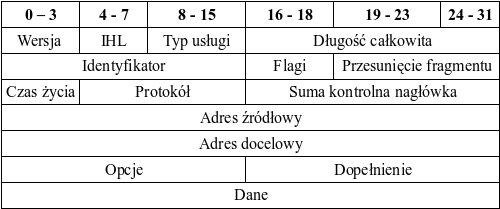
\includegraphics[scale=0.65]{ip-datagram.jpg}
					\caption{Datagram IPv4}
				\end{figure}
				\begin{description}
					\item[Wersja] - w tym polu nagłówka znajduje się wersja protokołu IP, w przypadku IPv4 znajduje się tam cyfra 4
					\item[IHL] - długość nagłówka pakietu IP wyrażona w postaci liczby czterobajtowych części
					\item[Typ usługi] – określa priorytet pakietu
					\item[Długość całkowita] – pole zawiera całkowitą długość pakietu (nagłówek + dane), maksymalna długość pakietu to 65535 bajtów
					\item[Identyfikator ]  – pole zawiera unikatory identyfikator dla każdego pakietu wykorzystywany do połączenia pakietów w strumień danych
					\item[Flagi] – określa między innymi czy pakiet może być fragmentowany
					\item[Przesunięcie fragmentu] – umożliwia złożenie pakietu w całość pakietu, określają miejsce danego fragmentu w całym pakiecie
					\item[Czas życia (TTL – Time To Live)] – ilość przeskoków przez które może pakiet przejść zanim zostanie odrzucony (urządzenia przez które przechodzi dany pakiet zmniejszają tą wartość o 1)
					\item[Protokół ] – to pole zawiera informacje jaki protokół warstwy transportowej został wykorzystany (TCP, UDP, ICMP lub inne)
					\item[Suma kontrolna nagłówka] – gdy odbiorca dostanie pakiet, sprawdza jego poprawność obliczając sumę kontrolną i porównując ją z sumą kontrolną zapisaną w nagłówku
					\item[Adres źródłowy i adres docelowy ] – zawierają adresy IP urządzeń które przesyłają między sobie dane zapisane w formacie binarnym
				\end{description}
			\newpage\subsection{\color{red}Ethernet.}
				a
			\newpage\subsection{\color{red}Protokoły warstwy aplikacji.}
				a
			\newpage\subsection{Charakterystyka modelu OSI i TCP/IP.}
				\begin{figure}[h!]
					\centering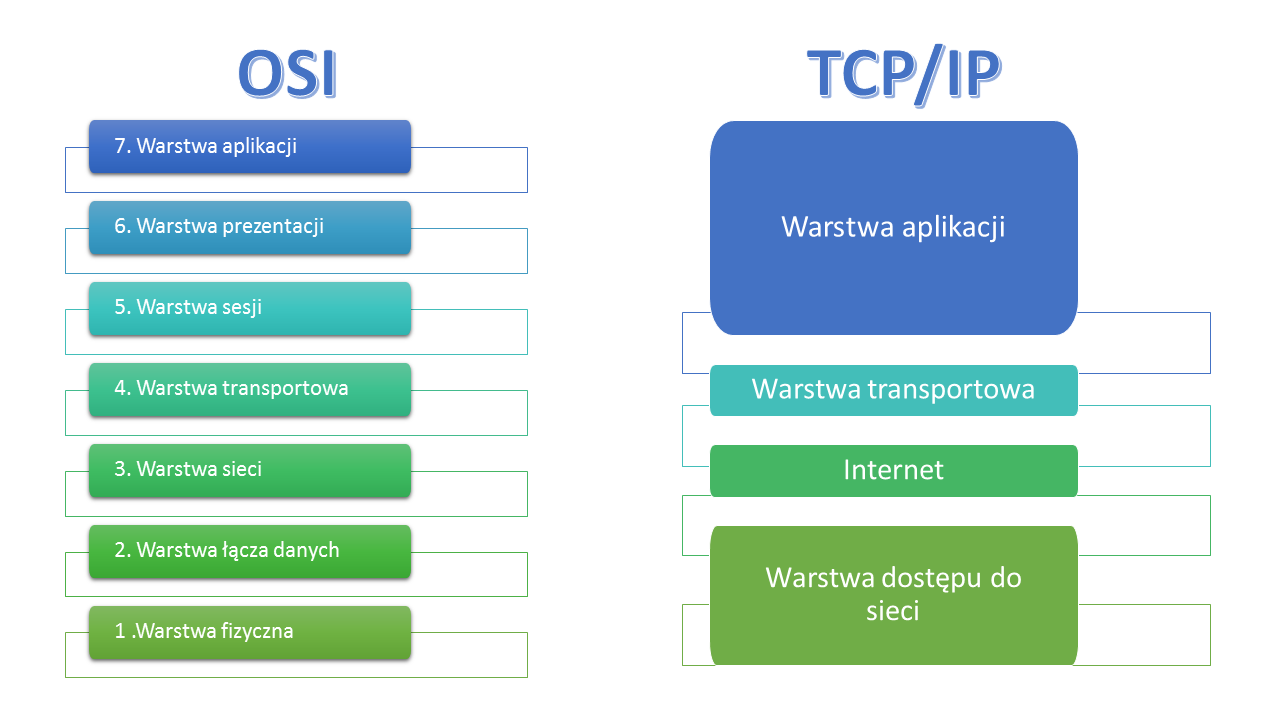
\includegraphics[scale=0.45]{osi-tcp.png}
					\caption{OSI - TCP/IP}
				\end{figure}
				\subsubsection{OSI}
				\subparagraph{Model ISO/OSI} (International Organization for Standardization / Open Systems
				Interconnection) - to standard opisujący komunikację sieciową oraz jej etapy. Jest on znany
				jako “model odniesienia” który służy do analizy (i zrozumienia) komunikacji.
				
				Warstwy:
				\begin{enumerate}
					\item \textbf{Warstwa fizyczna} - zaliczają się do niej wszystkie media transmisji danych (np.
					kable, fale radiowe) oraz sposób przesyłania przez nich informacji (np. jaka
					częstotliwość lub amplituda). 
					\item \textbf{Warstwa łącza danych} - przeprowadza ramkowanie danych (dodawanie nagłówka
					do danych) i przesyła je przez warstwę fizyczną. W nagłówku zawarty jest adres
					MAC nadawcy oraz odbiorcy (host zna adresy MAC swoich najbliższych sąsiadów).
					Przykładowy protokół: PPP, Ethernet, STP
					\item \textbf{Warstwa sieci} - w tej warstwie tworzone są pakiety (dane + nagłówek IP).
					Wykonywane jest tutaj adresowanie logiczne, routing oraz szukanie najlepszej
					ścieżki.\\
					Przykładowe protokoły: ARP, ICMP, IPv4, IPv6, BGP, RIP, OSPF
					\item \textbf{Warstwa transportowa} - tworzy ona segmenty danych (nagłówek zawierający
					numer portów + dane) i wykorzystuje do nich przesyłu przez protokół UDP lub TCP.
					Mogą tutaj występować mechanizmy zapewniające dostarczanie danych jak np.
					retransmisja (TCP ma, a UDP tego nie ma).\\
					Przykładowe protokoły: TCP, UDP, SSL/TLS
					\item \textbf{Warstwa sesji} - nie modyfikuje danych lecz zarządza ona sesją i synchronizacją
					danych. Mając jakieś dane wie ona do jakiej aplikacji przesłać te dane (umożliwia
					komunikację między aplikacjami [end-to-end]).\\
					Przykładowe protokoły: NetBIOS, NFS, PAP
					\item \textbf{Warstwa prezentacji} - polega na normalizacji danych według ustalonych
					standardów poprzez konwersję (zamianę), kompresję, szyfrowanie.\\
					Przykładowe protokoły: SSl, TLS, MIME
					\item \textbf{Warstwa aplikacji} - tutaj działają aplikacje które widzi użytkownik służące do
					przyjmowania i wyświetlania danych użytkownika oraz przy wykorzystaniu gniazd do
					przyjmowaniu danych z sieci i wysyłaniu danych do sieci\\
					Przykładowe protokoły: HTTP, FTP, POP3, SNMP
				\end{enumerate}
			
			\subsubsection{TCP/IP}
			\subparagraph{Model TCP/IP}- model określany inaczej jako “model protokołów”, gdzie każda warstwa
			wykonuje konkretne zadania.
			
			Warstwy:
			\begin{enumerate}
				\item \textbf{Warstwa dostępu do sieci} - służy ona do przekazywania danych między
				urządzeniami sieciowymi (karty sieciowe, modemy) za pośrednictwem medium
				fizycznym (np. kable)\\
				Odpowiada ona warstwie fizycznej i łącza danych z modelu OSI.
				\item \textbf{Warstwa internetu} - w tej warstwie występują routery opierające się o adresy IP i
				dokonujące trasowania (wyszukiwanie najlepszej trasy do odbiorcy).
				Występują tutaj protokoły takie jak: IP, ARP, ICMP (do diagnostyki), IGRP (do
				transmisji grupowej).\\
				Odpowiada ona warstwie sieci z modelu OSI.
				\item \textbf{Warstwa transportowa} - służy ona do obsługi komunikacji oraz jej zabezpieczenia
				(czyli wykorzystanie np. retransmisji danych). Ta warstwa wykorzystuje porty dzięki
				czemu wie z jakiej aplikacji przychodzą dane, a podczas odbierania do jakiej aplikacji
				przesłać dane. Występuje tutaj protokół TCP oraz UDP.\\
				Odpowiada ona warstwie transportowej z modelu OSI.
				\item \textbf{Warstwa aplikacji} - w tej warstwie występują procesy oraz aplikacje z których
				korzystają użytkownicy (np. serwer WWW, przeglądarka internetowa). Działają tutaj
				protokoły tj. HTTP, FTP, Telnet.\\
				Odpowiada ona warstwie sesji, prezentacji i aplikacji z modelu OSI.
			\end{enumerate}
			
			\newpage\subsection{\color{red}Rodzaje i przykłady nagłówków HTTP.}
				a
			\newpage\subsection{\color{red}Protokół WebSocket.}
				a
			\newpage\subsection{\color{red}Serwer zdarzeniowy, a wielowątkowy. Charakterystyka i porównanie.}
				a
		
		\newpage\section{Bezpieka}
			\subsection{\color{red}Infrastruktura klucza publicznego - charakterystyka.}
				a
			
			\newpage\subsection{Kryptografia symetryczna oraz asymetryczna - charakterystyka.}
				
				\subsubsection*{Kryptografia symetryczna}
				
				W kryptografii symetrycznej szyfrowanie i deszyfrowanie wykonywane jest przy użyciu tego samego klucza. W niektórych algorytmach wykorzystywane są dwa klucze, jednak muszą one być od siebie zależne w taki sposób, że znając jeden z nich, można wygenerować drugi.
				
				\begin{figure}[h!]
					\centering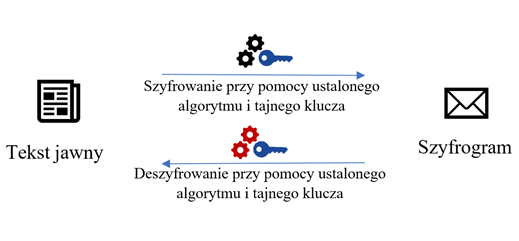
\includegraphics[scale=0.45]{krypt_sym.png}
					\caption{Zasada działania kryptografii symetrycznej}
				\end{figure}
				
				W celu zapewnienia bezpiecznej komunikacji, algorytm szyfrowania musi być tak skonstruowany, żeby odtworzenie tekstu jawnego bez znajomości klucza było zadaniem trudnym obliczeniowo. Dodatkowym wymaganiem jest tajność klucza – przed rozpoczęciem wymiany wiadomości, należy opracować protokół uzgadniania lub przekazywania klucza.
				
				Algorytmy szyfrowania symetrycznego możemy podzielić na algorytmy blokowe i strumieniowe. Pierwsze z nich przekształcają blok danych ustalonej długości, traktując go jako całość, na szyfrogram o tej samej liczbie bitów. Szyfry strumieniowe przyjmują natomiast ciąg (strumień) danych. Algorytmy kryptografii symetrycznej są szybkie, zwykle wymagają też mniejszej mocy obliczeniowej niż algorytmy asymetryczne. Powszechnie stosowanym szyfrem symetrycznych jest \textbf{AES}.
				
				\subsubsection*{Kryptografia asymetryczna}
				
				Kryptografia asymetryczna to rodzaj kryptografii, w którym jeden z używanych kluczy jest udostępniony publicznie. Każdy użytkownik może użyć tego klucza do zaszyfrowania wiadomości, ale tylko posiadacz drugiego, tajnego klucza może odszyfrować taką wiadomość.
				
				Kryptografia asymetryczna opiera się na funkcjach jednokierunkowych – takich, które da się łatwo wyliczyć w jedną stronę, ale bardzo trudno w drugą. Np. mnożenie jest łatwe, a rozkład na czynniki (z ang. faktoryzacja) trudny (na czym przykładowo opiera się \textbf{RSA}). Potęgowanie modulo jest łatwe, a logarytmowanie dyskretne jest trudne (na czym opierają się ElGamal, DSA i \textbf{ECC}).
				
				\begin{figure}[h]
					\centering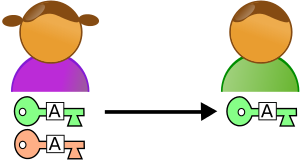
\includegraphics[scale=0.45]{krypt_asym_1.png}
					\caption{Krok 1: Alice przesyła do Boba swój klucz publiczny}
					
					\hspace{5pt}
					
					\centering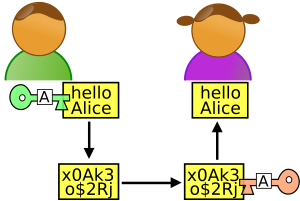
\includegraphics[scale=0.45]{krypt_asym_2.png}
					\caption{Kroki 2 i 3: Bob szyfruje wiadomość kluczem publicznym Alice, która to następnie otrzymuje zaszyfrowaną wiadomość i rozszyfrowuje ją kluczem prywatnym}
				\end{figure}
				
				Klucz publiczny używany jest do zaszyfrowania informacji, klucz prywatny do jej odczytu. Ponieważ klucz prywatny jest w wyłącznym posiadaniu adresata informacji, tylko on może ją odczytać. Natomiast klucz publiczny jest udostępniony każdemu, kto zechce zaszyfrować wiadomość.
				
				Ponieważ kryptografia asymetryczna jest o wiele wolniejsza od symetrycznej, prawie nigdy nie szyfruje się wiadomości za pomocą kryptosystemów asymetrycznych (również ze względu na ograniczenie wielkości szyfrowanej wiadomości). Zamiast tego szyfruje się jedynie klucz jakiegoś szyfru symetrycznego, takiego jak np. AES. Takie protokoły, łączące elementy kryptografii symetrycznej i asymetrycznej, nazywa się hybrydowymi.
				
				Nadawcy mogą także używać kluczy prywatnych do cyfrowego podpisywania wiadomości. Te podpisy cyfrowe pozwalają odbiorcom uwierzytelnić tożsamość nadawcy i spać spokojnie, wiedząc, że wiadomości nie zostały zmienione od momentu podpisania. W takim przypadku przesyłane informacje mogą być publiczne, a odbiorca może użyć certyfikatu, który towarzyszy tej informacji, aby zweryfikować integralność i autentyczność podpisanej wiadomości.
				
				\begin{figure}[h]
					\centering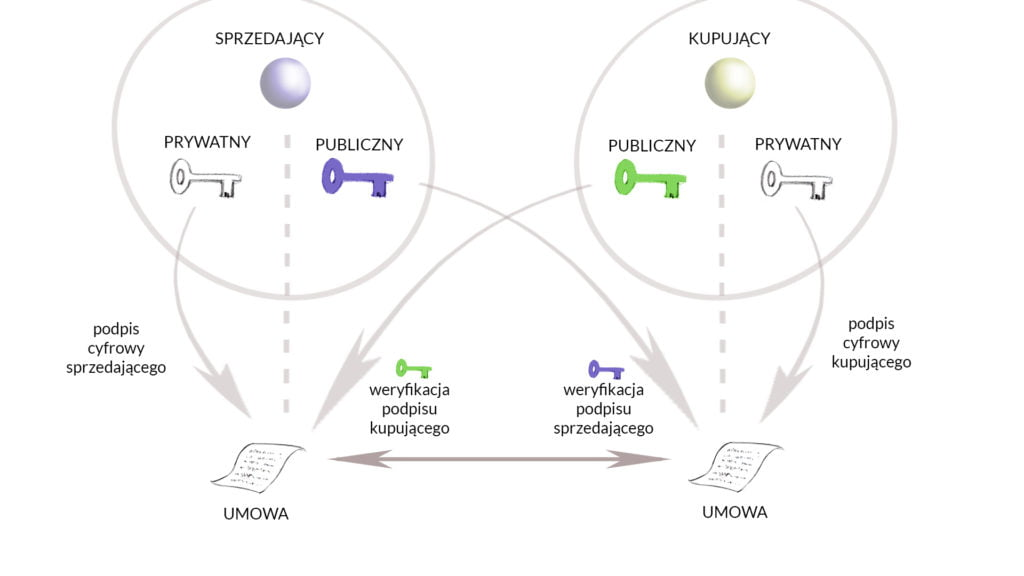
\includegraphics[scale=0.35]{krypt_asym_podpis.png}
					\caption{Jak działa podpis}
				\end{figure}
				
			\newpage\subsection{\color{red}Bezpieczeństwo sieci w odniesieniu do warstw modelu TCP/IP.}
				a
			\newpage\subsection{\color{red}Metody kontroli dostępu w systemach IT.}
				a
			\newpage\subsection{\color{red}Atrybuty bezpieczeństwa informacji.}
				a
	
	\chapter{Pytania - dr. hab. Grzegorz Wójcik}
	
		\section{Bazy danych}
			\subsection{Model relacyjny baz danych i języki zapytań.}
			
				\subsubsection{Model relacyjny baz danych}
				
				Relacyjny model danych pojawił się po raz pierwszy w artykule naukowym Edgara Codda w 1970 roku.
				W terminologii matematycznej - baza danych jest zbiorem relacji.  Stąd historycznie pochodzi nazwa relacyjny model danych i relacyjna baza danych. W matematyce definiuje się relację jako podzbiór iloczynu kartezjańskiego zbiorów wartości. Reprezentacją relacji jest dwuwymiarowa tabela złożona z kolumn i wierszy. \\ \\ Założenia modelu relacyjnego:
				\begin{itemize}
				\itemsep 0em
				\item Liczba \textbf{kolumn/atrybutów/pól (synonimy)} jest z góry ustalona.
				\item Z każdą kolumną jest związana jej nazwa (np. FirstName) oraz dziedzina (np. TEXT(20)), określająca zbiór wartości, jakie mogą wystąpić w kolumnie.
				\item Na przecięciu \textbf{wiersza/krotki/rekordu (synonimy)} i kolumny znajduje się pojedyncza (atomowa) wartość należąca do dziedziny kolumny.
				\item Wiersz reprezentuje jeden rekord informacji np. osobę.
				\item W modelu relacyjnym abstrahujemy od kolejności wierszy (rekordów) i kolumn (pól w rekordzie).
				\end{itemize}
				
				\noindent \textbf{Klucz główny}: dla każdej tabeli musi być określony klucz główny, będący jednoznacznym identyfikatorem. Może to być jedna lub więcej kolumn, w których wartości jednoznacznie identyfikują cały wiersz. Klucz główny w tabeli może być tylko jeden. \\
				\textbf{Klucz jednoznaczny} ma te same właściwości co klucz główny, ale ich może być w tabeli więcej niż jeden. \\
				\textbf{Klucz obcy} - jedna lub więcej kolumn, których wartości występują również jako klucz główny/jednoznaczny w tej samej/innej tabeli i są interpretowane jako wskaźniki do wierszy w tej drugiej tabeli
				
				\noindent \\ \textbf{Dwanaście postulatów Codda} – jest to zestaw 13 zasad stworzonych przez Edgara F. Codda – pioniera relacyjnych baz danych. Każda relacyjna baza danych musi je spełniać:
				\begin{itemize}
				\itemsep 0em
					\item System musi być kwalifikowany jako relacyjny, jako baza danych i jako system zarządzania.
					\item \textbf{Postulat informacyjny} – dane są reprezentowane jedynie przez wartości atrybutów w wierszach tabel (w krotkach).
					\item \textbf{Postulat dostępu} – każda wartość w bazie danych jest dostępna poprzez podanie nazwy tabeli, atrybutu i wartości klucza podstawowego (głównego).
					\item \textbf{Postulat dotyczący wartości NULL} – dostępna jest specjalna wartość NULL dla reprezentacji zarówno wartości nieokreślonej, jak i nieadekwatnej, inna od wszystkich i podlegająca przetwarzaniu.
					\item \textbf{Postulat dotyczący katalogu} – wymaga się, aby system obsługiwał wbudowany katalog relacyjny z bieżącym dostępem dla uprawnionych użytkowników używających języka zapytań.
					\item \textbf{Postulat języka danych} – system musi dostarczać pełny język przetwarzania danych, który może być używany zarówno w trybie interaktywnym, jak i w obrębie programów, obsługuje operacje definiowania danych, operacje manipulowania danymi, ograniczenia związane z bezpieczeństwem i integralnością oraz operacje zarządzania transakcji.
					\item \textbf{Postulat modyfikowalności perspektyw} – system musi umożliwiać modyfikowanie perspektyw, o ile jest ono semantycznie realizowalne.
					\item \textbf{Postulat modyfikowalności danych} – system musi umożliwiać operacje modyfikacji danych, musi obsługiwać operacje INSERT, UPDATE oraz DELETE.
					\item \textbf{Postulat fizycznej niezależności danych} – zmiany fizycznej reprezentacji danych i organizacji dostępu nie wpływają na aplikacje.
					\item \textbf{Postulat logicznej niezależności danych} – zmiany wartości w tabelach nie wpływają na aplikacje.
					\item \textbf{Postulat niezależności więzów spójności} – więzy spójności są definiowane w bazie i nie zależą od aplikacji.
					\item\textbf{ Postulat niezależności dystrybucyjnej} – działanie aplikacji nie zależy od modyfikacji  i dystrybucji bazy.
					\item \textbf{Postulat bezpieczeństwa względem operacji niskiego poziomu} – operacje niskiego poziomu nie mogą naruszać modelu relacyjnego i więzów spójności.
				\end{itemize}
				
			\noindent Operacje modelu relacyjnego:
			\begin{itemize}
				\itemsep 0em
				\item Selekcja - \verb*|WHERE| - selekcja podzbioru wierszy które spełniają określone warunki
				\item Projekcja - \verb*|SELECT| - pominięcie z wyniku pewnych kolumn
				\item Opracje na zbiorach: iloczyn kartezjański - \verb*|FROM| (złączenie tabel), suma zbiorów - \verb*|UNION|, różnica zbiorów - \verb*|EXCEPT|
				\item Agregacja - funkcje agregujące \verb*|SUM|, \verb*|MIN| itd. oraz klauzula \verb*|GROUP BY|
			\end{itemize}
			
			\newpage \subsubsection{Języki zapytań}
			\textbf{SQL} - Structured Query Language - jest to język strukturalny (i deklaratywny) służący do zarządzania bazą danych (CRUD). SQL jest najbardziej znanym językiem zapytań, ale istnieje także xBase.
			
			\begin{itemize}
			\item \textbf{DML (Data Manipulation Language)} służy do wykonywania operacji na danych – do ich umieszczania w bazie, kasowania, przeglądania oraz dokonywania zmian. Najważniejsze polecenia z tego zbioru to:
			\subitem \verb*|INSERT| – umieszczenie danych w bazie,
			\subitem \verb*|UPDATE| – zmiana danych,
			\subitem \verb*|DELETE| – usunięcie danych z bazy.
			
			\item \textbf{DDL (Data Definition Language)} - operacje na strukturach, w których dane są przechowywane – czyli np. dodawanie, zmienianie i kasowanie tabel lub baz. Najważniejsze polecenia tej grupy to:
			
			\subitem \verb*|CREATE| – utworzenie struktury (bazy, tabeli, indeksu itp.)
			\subitem \verb*|DROP| – usunięcie struktury
			\subitem \verb*|ALTER| – zmiana struktury

			\item \textbf{DCL (Data Control Language)} ma zastosowanie do nadawania uprawnień do obiektów bazodanowych. Najważniejsze polecenia w tej grupie to:
			
			\subitem \verb*|GRANT| – nadawanie uprawnień do pojedynczych obiektów lub globalnie konkretnemu użytkownikowi
			\subitem \verb*|REVOKE| – odbieranie wskazanych uprawnień konkretnemu użytkownikowi
			\subitem \verb*|DENY| – zabranianie wykonywania operacji

			\item \textbf{DQL (Data Query Language}) to język formułowania zapytań do bazy danych. W zakres tego języka wchodzi jedno polecenie – \verb*|SELECT|. Często SELECT traktuje się jako część języka DML, ale to podejście nie wydaje się właściwe, ponieważ DML z definicji służy do manipulowania danymi – ich tworzenia, usuwania i uaktualniania. Na pograniczu obu języków znajduje się polecenie SELECT INTO, które dodatkowo modyfikuje (przepisuje, tworzy) dane.
			\end{itemize}
				
				
			\newpage\subsection{\color{green} Paweł \color{red}Model obiektowo-relacyjny baz danych, inne modele danych.}
				a
			\newpage\subsection{Składnia podstawowych zapytań języka SQL.}
				\subsubsection{DDL - Data Definition Language}
				\noindent Jak zapamiętać skrót: \\ Definition = DEFINIOWANIE - TWORZENIE STRUKTUR \\
				\noindent W skład DDL wchodzą \verb*|DROP|, \verb*|CREATE| oraz \verb*|ALTER|.
				\begin{itemize}
					\itemsep 0em
					\item \verb*|DROP| - usunięcie struktury
					\begin{verbatim}
						DROP TABLE tabela;
					\end{verbatim}
					\item \verb*|CREATE| - stworzenie struktury
					\begin{verbatim}
						CREATE TABLE tabela(
							kolumna1 typ (rozmiar),
							kolumna2 typ (rozmiar),
							...
						);
					\end{verbatim}
					\item \verb*|ALTER| - modyfikacja struktury. Obejmuje operacje takie jak np. dodanie kolumny do tabeli, zmiana typu danych w kolumnie, usunięcie kolumny.
					\begin{verbatim}
						ALTER TABLE table
						ADD kolumna typ(dlugosc);
					\end{verbatim}
					\begin{verbatim}
						
					\end{verbatim}
				\end{itemize}
				
				
				\subsubsection{DML - Data Manipulation Language}
				\noindent Jak zapamiętać skrót: \\ Manipulation = MANIPULACJA - EDYCJA LUB TWORZENIE REKORDÓW \\
				\noindent W skład DML wchodzą \verb*|INSERT|, \verb*|UPDATE| oraz \verb*|DELETE|.
				\begin{itemize}
					\itemsep 0em
					\item \verb*|INSERT| - dodawanie wierszy
					\begin{verbatim}
						INSERT INTO tabela (kolumna1, kolumna2, ..., kolumna_n)
						VALUES (wartosc1, wartosc2, ..., wartosc_n)
					\end{verbatim}
					Nie trzeba podawać kolumn po nazwie tabeli gdy podamy po pierwsze wszystkie wartości, a po drugie w dobrej kolejności
					
					\item \verb*|UPDATE| - aktualizowanie danych, zmiana
					\begin{verbatim}
						UPDATE tabela
						SET kolumna1 = wartosc, kolumna2 = wartosc2, ...
						WHERE warunek
					\end{verbatim}
					WHERE nie jest konieczny, możemy  go użyć jak chcemy doprecyzować które rekordy mają się zaktualizować
					
					\item \verb*|DELETE| - usuwanie wierszy
					\begin{verbatim}
						DELETE FROM tabela
						WHERE warunek
					\end{verbatim}
					WHERE nie jest konieczny, możemy  go użyć jak chcemy doprecyzować które rekordy mają się skasować
				\end{itemize}
				\subsubsection{DCL - Data Control Language}
				\noindent Jak zapamiętać skrót: \\ Control = KONTROLA = UPRAWNIENIA \\
				\noindent W skład DCL wchodzą \verb*|GRANT|, \verb*|REVOKE| oraz \verb*|DENY|.
				
				\begin{itemize}
					\item \verb*|GRANT| - nadawanie uprawnień do pojedynczych obiektów lub globalnie konkretnemu userowi
					\item \verb*|REVOKE| - odbieranie uprawnień konkretnemu userowi
					\item \verb*|DENY| - zabranianie wykonywania operacji
					\item Składnia jest taka sama dla w/w poleceń:
					\begin{verbatim}
						[GRANT/REVOKE/DENY] operacja1, operacja2, ...
						ON tabela
						TO user
					\end{verbatim}
					Przykład:
					\begin{verbatim}
					GRANT SELECT, INSERT
					ON Fragment
					TO glazik
					\end{verbatim}
				\end{itemize}
				
				\subsubsection{DQL - Data Query Language}
				\noindent Jak zapamiętać skrót: \\ Query = ZAPYTANIA = SELECTY \\
				\noindent W skład DQL wchodzi jedno polecenie: \verb*|SELECT|. Pozwala wybierać wiersze z bazy danych. Składnia:
				\begin{verbatim}
					SELECT kolumny 
					FROM tabele 
					WHERE warunek
					GROUP BY kolumna
					HAVING warunek
					ORDER BY ... DESC/ASC;
				\end{verbatim}
				Dodatkowe klauzule \verb*|SELECT|:
				\begin{itemize}
					\itemsep 0em
					\item \verb*|ORDER BY| - sortowanie wyników względem np. kolumny
					\item \verb*|ASC| oraz \verb*|DESC| - dodawane po sortowaniu, wybieramy czy ma być ascending czy descending
					\item \verb*|GROUP BY| - grupowanie wyników względem danej kolumny
					\item \verb*|HAVING| - filtrowanie grup, działa podobnie do WHERE. WHERE oraz HAVING mogą występować jednocześnie w zapytaniu.
				\end{itemize}
				
			\newpage\subsection{Projektowanie baz danych oraz model związków encji.}
			\subsubsection{Projektowanie baz danych}
				Etapy projektowania systemów bazodanowych:
				\begin{itemize}
					\item \textbf{Sformułowanie problemu}
					\item \textbf{Analiza wycinka rzeczywistości} - wywiad z ekspertem dziedzinowym, analiza wymagań funkcjonalnych (co dodawać, co usuwać itd.) i niefunkcjonalnych (tryb graficzny, platforma sprzętowa itd.)
					\item \textbf{Opracowanie konceptualnego modelu danych}, czyli wyodrębnienie i zdefiniowanie encji, związków między nimi oraz atrybutów (taka jakby luźna forma) \\
					Projektowanie modelu konceptualnego bazy danych składa się z następujących etapów:
					\begin{itemize}
						\item \textbf{określenie zbiorów encji} - jakie encje (tabele) będzie zawierać baza?
						\item \textbf{określenie atrybutów encji} - jakie cechy (kolumny) będą miały poszczególne encje?
						\item \textbf{określenie dziedziny atrybutów} - jaki zakres wartości będzie miał każdy atrybut?
						\item \textbf{ustalenie kluczy podstawowych} - a'la klucze główne (?)
						\item \textbf{określenie związków między encjami} - a'la klucze obce (?)
					\end{itemize}
					\textbf{Encja} to każdy element rzeczywistości, który można scharakteryzować i odróżnić od innych obiektów, np. książka (przedmiot), klient (obiekt), zamówienie (zjawisko), stan cywilny (stan). \\
					\textbf{Atrybut} to cecha encji. Zestaw atrybutów, które określamy dla encji, zależy od potrzeb bazy danych (np. książka ma atrybuty: tytuł, autor, ...) \\
					\textbf{Dziedzina} opisuje jakie wartości może przyjąć dany atrybut, np. tytuł książki to napis o długości do x znaków.
					\item \textbf{Opracowanie modelu logicznego}, czyli wyrażenie świata rzeczywistego za pomocą reguł modelu danych (np. relacyjnego). Transformujemy model konceptualny do logicznego. Zamiast encji są tabele, zamiast związków są wiązania poprzez klucze główne i obce itd. Następuje normalizacja relacji.
					\item \textbf{Opracowanie modelu fizycznego}, czyli konstruowanie modelu świata rzeczywistego za pomocą struktur danych i mechanizmów istniejących w wybranym SZBD (systemie zarządzania bazami danych), czyli np naklepanie tego w MySQL
					\item \textbf{Tworzenie aplikacji}
					\item \textbf{Testowanie systemu}
				\end{itemize}
				
			\newpage
			\subsubsection{Model związków encji}
			\noindent  Model związków encji (model ER lub ERD) to jedna z najpopularniejszych metod modelowania danych. Służy do graficznego przedstawiania koncepcji projektowanej bazy danych. Jest bardzo podobny do relacyjnego modelu. Diagram taki pokazuje obiekty (encje), ich cechy (atrybuty) oraz relacje między nimi. Elementy takie, jak encja, atrybut oraz związek zostały opisane stronę wyżej. \\ \\
			Typy związków encji:
			\begin{itemize}
				\itemsep 0em
				\item \textbf{jeden do jednego} (1:1) \\
				Związek ten określa, iż każde wystąpienie danego obiektu (encji) związane jest wyłącznie z pojedynczym wystąpieniem innego bytu. Na przykład: Pracownik w organizacji ma przypisane konkretne Miejsce, a to Miejsce jest przypisane do konkretnego Pracownika. Kierownik zarządza jednym Działem, a Dział zarządzany jest przez jednego Kierownika.
				\item \textbf{jeden do wielu} (1:N) \\
				Związek ten określa, iż jedno wystąpienie danego obiektu (encji) związane jest z większą ilością wystąpień innego bytu. Na przykład: Klient składa wiele Zamówień. Konkretne Zamówienie jest składane przez danego Klienta. W Firmie istnieje wiele Działów. Konkretny Dział istnieje w danej Firmie.
				\item \textbf{wiele do wielu} (M:N) \\
				Związek ten określa, iż jedno wystąpienie danego obiektu (encji) związane jest z większą ilością wystąpień innego bytu, tak samo jak jedno wystąpienie innego bytu może być powiązane z większą ilością wystąpień tego pierwszego obiektu. Przykładem takiego związku może być zależność jaka występuje pomiędzy Studentem oraz Wykładem. Student zapisany może być na wiele Wykładów, tak i na dany Wykład zapisanych może być wielu Studentów.
			\end{itemize}
			
			\newpage\subsection{\color{green} Paweł \color{red}Problemy indeksowania baz danych, rodzaje indeksów, indeksy typu B+ drzewo.}
				a
			\newpage\subsection{Przetwarzanie transakcyjne OLTP (On-Line Transaction Processing).}
		\textbf{OLTP} (Online Transaction Processing) to kategoria aplikacji klient-serwer dotyczących baz danych w ramach bieżącego przetwarzania transakcji obejmujących takie zastosowania jak systemy rezerwacji, obsługa punktów sprzedaży, systemy śledzące itp. W systemach tych klient współpracuje z serwerem transakcji, zamiast z serwerem bazy danych.  Zastosowanie - np. w bankowości internetowej, w handlu detalicznym, podczas składania zamówień lub przy wysyłaniu wiadomości tekstowych. Transakcje te (tradycyjnie określane jako transakcje gospodarcze lub finansowe) są rejestrowane i zabezpieczane w taki sposób, aby przedsiębiorstwo mogło w każdej chwili uzyskać do nich dostęp w celach księgowych lub sprawozdawczych. \\

		System OLTP:
		\begin{itemize}
			\itemsep 0em
			\item Umożliwia wykonywanie w czasie rzeczywistym dużej liczby transakcji bazodanowych przez dużą liczbę osób
			\item Wymaga błyskawicznych czasów reakcji
			\item Często modyfikuje małe ilości danych i zazwyczaj dokonuje tyle samo odczytów, co zapisów danych
			\item Używa indeksowanych danych w celu skrócenia czasu odpowiedzi
			\item Wymaga częstego lub równoczesnego wykonywania kopii zapasowych bazy danych
			\item Wymaga stosunkowo niewiele miejsca do przechowywania danych
			\item Zazwyczaj obsługuje proste zapytania dotyczące tylko jednego lub kilku rekordów
		\end{itemize}
		
		\textbf{Transakcja} to zbiór operacji na bazie danych, które stanowią w istocie pewną całość i powinny być wykonane wszystkie lub żadna z nich. Składa się zawsze z trzech etapów: \textbf{rozpoczęcia, wykonania i zamknięcia}. W systemach bazodanowych istotne jest, aby trwała jak najkrócej, ponieważ równolegle może być wykonywane wiele transakcji i część operacji musi zostać wykonana w pewnej kolejności. Każdy etap transakcji jest logowany, dzięki czemu w razie awarii można odtworzyć stan bazy sprzed transakcji. \\
		Cechy transakcji: \textbf{ACID} \\
		- \textbf{A}tomicity - atomowość - wykona się wszystko albo nic (zbiór operacji = całość); \\
		- \textbf{C}onsistency - spójność - baza przed i po zmianach jest spójna; \\
		- \textbf{I}solation - izolacja - równolegle wykonywane transakcje nie mają na siebie wpływu; \\
		- \textbf{D}urability - trwałość - zmiany prowadzone przez transakcje są trwałe (nawet w przypadku awarii);\\
		W SQL wyróżniamy następujące polecenia dotyczące transakcji:
		\begin{itemize}
			\itemsep 0em
			\item \verb*|BEGIN| lub \verb*|BEGIN WORK| – rozpoczęcie transakcji
			\item \verb*|COMMIT| – zatwierdzenie zmian wykonanych w obrębie transakcji
			\item \verb*|ROLLBACK| – odrzucenie zmian wykonanych w obrębie transakcji
			\item \verb*|SAVEPOINT nazwa| – zdefiniowanie punktu pośredniego o określonej nazwie
			\item \verb*|RELEASE SAVEPOINT nazwa| – skasowanie punktu pośredniego (nie wpływa w żaden sposób na stan transakcji)
			\item \verb*|ROLLBACK TO SAVEPOINT nazwa| – wycofanie transakcji do stanu zapamiętanego w podanym punkcie pośrednim.
		\end{itemize}
		\newpage\section{Paradygmaty}
			\subsection{\color{red}Założenia paradygmatu programowania obiektowego.}
				a
			\newpage\subsection{\color{green} Rafał \color{red}Idea dziedziczenia i polimorfizmu w programowaniu.}
				a
			\newpage\subsection{\color{red}Zasady programowania dynamicznego.}
				a
			\newpage\subsection{\color{green} Rafał \color{red}Główne paradygmaty programowania.}
				a
			\newpage\subsection{\color{green} Rafał \color{red}Cechy programowania deklaratywnego.}
				a
	
	\chapter{Pytania - reszta}
	
		\section{Jezyk C i C++}
			\subsection{\color{red}Instrukcje sterujące w języku C.}
				a
			\newpage\subsection{\color{red}Zarządzanie pamięcią w języku C.}
				a
			\newpage\subsection{\color{red}Budowa, obsługa i formatowanie łańcuchów znakowych w języku C.}
				a
			\newpage\subsection{\color{red}Zasięg i czas życia obiektów w języku C++.}
				a
			\newpage\subsection{\color{red}Obsługa wyjątków w języku C++.}
				a
			\newpage\subsection{\color{red}Definicje obiektu, klasy i szablonu klasy w języku C++.}
				a
		
		\newpage\section{Algosy}
			\subsection{\color{red}Algorytmy sortujące.}
				a
			\newpage\subsection{\color{red}Algorytmy zachłanne.}
				a
			\newpage\subsection{\color{red}Metoda ,,dziel i zwyciężaj'' konstruowania algorytmów.}
				a
			\newpage\subsection{\color{red}Struktura kopców binarnych.}
				a
			\newpage\subsection{\color{red}Algorytmy wyszukiwania najkrótszej ścieżki w grafie.}
				a
			\newpage\subsection{\color{red}Sposoby implementacji słownika.}
				a
			\newpage\subsection{\color{red}Tablice mieszające.}
				a
			\newpage\subsection{\color{red}Algorytmy Monte Carlo oraz algorytmy Las Vegas.}
				a
			\newpage\subsection{\color{red}Metody rozwiązywania rekurencji. Rekurencje Flawiusza i wieża w Hanoi.}
				a
			\newpage\subsection{\color{red}Algorytmy Euklidesa. Algorytmy faktoryzacji.}
				a
			\newpage\subsection{\color{red}Metody reprezentacji grafów w komputerze.}
				a
			\newpage\subsection{\color{red}Droga i cykl Eulera. Droga i cykl Hamiltona.}
				a
			\newpage\subsection{\color{red}Drzewo spinające graf.}
				a
		
		\newpage\section{Teoria obliczalności czy coś}
			\subsection{\color{red}Pojęcia P, NP, NP-zupełne.}
				a
		
		\newpage\section{Automaty i inne takie}
			\subsection{\color{red}Deterministyczne i niedeterministyczne automaty skończone.}
				a
			\newpage\subsection{\color{red}Automaty z epsilon przejściami, wyrażenia regularne.}
				a
			\newpage\subsection{\color{red}Kompilacja: gramatyka bezkontekstowa, skaner, parser, błędy.}
				a
		
		\newpage\section{Podstawy komputera i systemy operacyjne}
			\subsection{\color{red}Systemy liczbowe i konwersje pomiędzy nimi.}
			
				a
				
			\newpage\subsection{Sposoby cyfrowej reprezentacji liczby całkowitej i rzeczywistej.}
			
				\subsubsection{Liczby całkowite}
				
				\subparagraph{Kod \text{ZM} (kod znak-moduł)}
				
				Sprawa w kodzie ZM jest w miarę prosta i klarowna. Najstarszy bit $b_{n-1}$ dla n-bitowej liczby jest bitem znaku i określa czy liczba jest dodatnia czy ujemna:
				\begin{itemize}
					\item 0 - liczba dodatnia,
					\item 1 - liczba ujemna.
				\end{itemize}
				
				Bity od $b_{n-1}$ do $b_0$ odpowiadają za kodowanie wartości samej liczby. Wzór na obliczenie wartości liczby zakodowanej w \textbf{ZM}:
				\begin{center}
					$L_{ZM} = (-1)^{b_{n-1}} \cdot (b_{n-2}2^{n-2} + ... + b_22^2 + b_12^1 + b_02^0)$
				\end{center}
				
				Przykładowe kodowanie liczby na ośmiu bitach w kodzie \textbf{ZM}:
				\begin{center}
					$26 \longrightarrow \textbf{0}0011010 $\\
					$-26 \longrightarrow \textbf{1}0011010 $
				\end{center}
				
				Proste, logiczne, fajne. Pytania, problemy? To jedziemy dalej.
				
				
				\subparagraph{Kod \textbf{U2} (kod uzupełnień do 2)}
				
				Tutaj sprawa się nieco komplikuje z zapisem liczb ujemnych. Bit $b_{n-1}$ ma wagę $-2^{n-1}$ co sprawia, że musimy bitowo tak jakby zapisać odwrotność liczby, którą chcemy reprezentować jako ujemna (i dodać 1, żeby się wszystko zgadzało). W zapisie liczb dodatnich zapis jest identyczny jak w \textbf{ZM} - na najstarszym bicie musimy tylko zachować $0$.
				
				Istnieje prosty algorytm konwersji na U2 z wykorzystaniem ZM:
				\begin{enumerate}
					\item Zapisać moduł liczby w ZM,
					\item Dokonać inwersji bitów (0 na 1 i 1 na 0),
					\item Zwiększ wynik dodając 1.
				\end{enumerate}
				
				Przykład z liczbą -27 na 8 bitach:
				
				\begin{tikzpicture}[x=2.2cm,y=1.4cm]
					\node[text width=5cm] at (0, 0)   (a) {Zapisujemy liczbę 27 w ZM};
					\node[text width=3cm] at (0.5, 1)   (b) {$00011011$};
					\draw [-to] (0,0.2) -- (0.2,0.7);
					\node[text width=3cm] at (2, 1)   (b) {$11100100$};
					\node[text width=3cm] at (3.5, 1)   (b) {$\textbf{11100101}$};
					
					\draw [-to] (0.7,1) -- (1.2,1);
					\draw [-to] (2.2,1) -- (2.7,1);
					
					\node[text width=5cm] at (2, 2)   (a) {Odwracamy bity};
					\draw [-to] (1.7,1.8) -- (1.7,1.2);
					
					\node[text width=5cm] at (3.9, 0)   (a) {Dodajemy 1};
					\draw [-to] (3.2,0.2) -- (3.2,0.7);
				\end{tikzpicture}
				
				\subsubsection{Liczby rzeczywiste}
				
				\subparagraph{Zapis stałopozycyjny}
				
				Do zapisu liczby stałoprzecinkowej przeznaczona jest z góry określona liczba bitów, a pozycję przecinka ustala się
				arbitralnie, w zależności od wymaganej dokładności, wolne bity uzupełniając zerami. Do reprezentacji liczb ze
				znakiem stosuje także kod U2.
				
				Liczba $6,25=110,01_{(2)}$ zapisana na 8 bitach gdy częśd ułamkowa zajmuje 3 najmłodsze bity, ma postać:
				\begin{center}
					\begin{tikzpicture}[x=2.2cm,y=1.4cm]	
						\node[text width=3cm] at (0, 0)   (b) {$\underbrace{00110}_{\text{część całkowita}}$};
						\node[text width=3cm] at (0.39, 0.42)   (b) {$\overbrace{010}^{\text{część ułamkowa}}$};
					\end{tikzpicture}
				\end{center}
				
				A w reprezentacji U2 będzie miała postać:
				
				\begin{center}
					$11001110$
				\end{center}
				
				Część całkowita liczby zachowuje się identycznie jak w przypadku zwykłych liczb całkowitych, natomiast bity w części ułamkowej posiadają wagi $2^{-1}$, $2^{-2}$, itd. - czyli $\frac{1}{2}$, $\frac{1}{4}$, ..., więc ilość bitów w części ułamkowej wpływa na precyzję zapisu.
				
				\subparagraph{Zapis zmiennopozycyjny}
				
				Liczba zmiennoprzecinkowa jest komputerową reprezentacją liczb rzeczywistych zapisanych w postaci wykładniczej
				o podstawie 2. Przykładowa notacja:
				
				\begin{center}
					$(-1)^Z \cdot M \cdot 2^C = (-1)^Z \cdot (1+m) \cdot 2^{c - BIAS}$
				\end{center}
				gdzie:
				\begin{description}
					\item[$(-1)^Z$] - znak liczby
					\item[$M=1+m$] - znormalizowana mantysa (liczba spełniająca warunek: $1 \leq M \leq 2$). Ponieważ przed przecinkiem stoi zawsze 1, więc można ją przedstawić w postaci $1+m$, gdzie \emph{m} jest liczbę ułamkową: $0 \leq m \leq 1$)
					\item[$C=c-BIAS$] - cecha (liczba całkowita), która dzięki zastosowaniu stałej BIAS pozwoli przedstawid cechę w postaci
					różnicy c-BIAS (c jest liczbą całkowitą dodatnią, tzw spolaryzowana cechę)
					\item[$BIAS$] - stała (liczba całkowita BIAS zależna od danej implementacji – rozwiązuje problem znaku cechy)
				\end{description}
				Kodujemy wyłącznie:
				\begin{description}
					\item[z] - bit znaku
					\item[m] - mantysę pomniejszoną o 1
					\item[c] - cechę przesuniętą o BIAS
				\end{description}
				
				Załóżmy, że operujemy następującym zmiennopozycyjnym formatem zapisu liczby rzeczywistej:
				\begin{itemize}
					\item na zapis przeznaczamy 16 bitów
					\item najstarszy bit ($b_{15}$) to bit znaku (będziemy stosowad kod ZM)
					\item kolejne 6 bitów ($b_{9}$-$b_{14}$) to mantysa
					\item pozostałe bity ($b_0$-$b_8$) są przeznaczone na zapis cechy i przyjmijmy, że BIAS=9
				\end{itemize}
				
				Przedstawimy liczbę +0,0224609375 w powyższym formacie. Naszą liczbę zapisujemy w systemie binarnym w
				postaci wykładniczej o podstawie 2, przesuwamy przecinek zapisując ją w notacji wykładniczej:
				
				\begin{center}
					$0,0224609375 = 0,0000010111_{(2)} = 1,0111_{(2)} \cdot 2^{-6}$
				\end{center}
				
				Z tego wynika, że:
				
				\begin{itemize}
					\item Znak: $(-1)^0$
					\item Mantysa: $1.\textbf{\underline{0111}}_2$
					\item Cecha: $-6 = 3-9 = 11_2 - BIAS$
				\end{itemize}
				
				Oto liczba 0,0224609375 zapisana w zadanym formacie:
				\begin{center}
					\begin{tikzpicture}[x=2.2cm,y=1.4cm]	
						\node[text width=3cm] at (0, 0)   (b) {$\underbrace{0}_{\text{bit znaku}}$};
						\node[text width=3cm] at (0.38, 0.39)   (b) {$\overbrace{011100}^{\text{mantysa}}$};
						\node[text width=3cm] at (1, 0)   (b) {$\underbrace{000000011}_{\text{cecha}}$};
					\end{tikzpicture}
				\end{center}
			
			\newpage\subsection{\color{red}Wielowarstwowa organizacja oprogramowania komputera.}
				a
			\newpage\subsection{\color{red}Procesy, zasoby i wątki.}
				a
			\newpage\subsection{\color{red}Planowanie przydziału procesora, priorytety, wywłaszczanie oraz planowanie.}
				a
			\newpage\subsection{\color{red}Zarządzanie pamięcią operacyjną.}
				a
			\newpage\subsection{\color{red}Problem zakleszczenia, algorytm Bankiera.}
				a
		
		\newpage\section{Inżynieria Oprogramowania}
			\subsection{\color{red}Standardowe metodyki procesu wytwórczego oprogramowania.}
				a
			\newpage\subsection{\color{red}Metodyki zwinne (agile).}
				a
			\newpage\subsection{\color{red}Metody testowania oprogramowania.}
				a
			\newpage\subsection{\color{red}Walidacja i weryfikacja oprogramowania.}
				a
			\newpage\subsection{\color{red}Diagramy UML (przypadków użycia, klas, aktywności, sekwencji, stanów, obiektów, wdrożenia).}
				a
			\newpage\subsection{\color{red}Wzorce projektowe programowania obiektowego.}
				a
			\newpage\subsection{\color{red}Wzorce architektoniczne.}
				a
		
		\newpage\section{Systemy wbudowane i elektronika}
			\subsection{\color{red}Różnice pomiędzy obsługą zdarzeń w przerwaniach sprzętowych a obsługą zdarzeń w pętli programowej.}
				a
			\newpage\subsection{\color{red}Stosowalność systemów opartych o mikrokontrolery vs stosowalność typowych komputerów (stacjonarnych i laptopów).}
				a
			\newpage\subsection{\color{red}Dekoder, multiplekser i demultiplekser: budowa, zasada, działania, przeznaczenie/zastosowanie.}
				a
			\newpage\subsection{\color{red}Podstawowe układy budujące system mikroprocesorowy i sposób wymiany informacji pomiędzy nimi.}
				a
\end{document}